% This is a model template for the solutions in computational science. You can find a very useful documentation for LaTeX in Finnish at ftp://ftp.funet.fi/pub/TeX/CTAN/info/lshort/finnish/ or in English at ftp://ftp.funet.fi/pub/TeX/CTAN/info/lshort/english/. The section List of mathematical symbols in Chapter 3 is especially useful for the typesetting of mathematical formulas.

% Compile the document to PDF by command 'pdflatex model.tex' in the terminal. The command must be run twice for the references in the text to be correct.

\documentclass[a4paper,11pt]{article}
\usepackage[utf8]{inputenc}
% This includes letters such as � and �
\usepackage[T1]{fontenc}
% Use here 'Finnish' for Finnish hyphenation. You may have to compile the code twice after the change. 
\usepackage[english]{babel}
\usepackage{graphicx}
% Some math stuff
\usepackage{amsmath,amsfonts,amssymb,amsbsy,commath,booktabs,hyperref}  
% This is just to include the urls
\usepackage{hyperref}
\usepackage[margin=2cm]{geometry}

\setlength{\parindent}{0mm}
\setlength{\parskip}{1.0\baselineskip}

\usepackage{listings}
\usepackage{color}
\usepackage{pdfpages}

\definecolor{dkgreen}{rgb}{0,0.6,0}
\definecolor{gray}{rgb}{0.5,0.5,0.5}
\definecolor{mauve}{rgb}{0.58,0,0.82}

\lstset{frame=tb,
	language=Python,
	aboveskip=3mm,
	belowskip=3mm,
	showstringspaces=false,
	columns=flexible,
	basicstyle={\tiny\ttfamily},
	numbers=none,
	numberstyle=\tiny\color{gray},
	keywordstyle=\color{blue},
	commentstyle=\color{dkgreen},
	stringstyle=\color{mauve},
	breaklines=true,
	breakatwhitespace=true,
	tabsize=4
}

\begin{document}

\title{Becs-114.1100 Computational Science -- exercise round 7} % Replace the exercise round number
\author{Kunal Ghosh, 546247} % Replace with your name and student number
\maketitle
\section{Solution to Question 3}
\subsection{Determining a polynomial regressor to fit a given dataset}\label{prob3a}
In this exercise we are required to fit a polynomial regressor to a given dataset. The dataset can be found in Table 1. 
\begin{table}[ht]
\centering
\label{initial-label}
\begin{tabular}{|c|c|}
\hline
 \textbf{x}&\textbf{y} \\ \hline
-9.7 & 3.76 \\
-7.3 & 1.78 \\
-5.4 & 1.52 \\
-5.0 & 1.31 \\
-3.01 & 0.31 \\
-2.13 & 0.23 \\
-1.2 & 0.45 \\
-0.56 & 0.29 \\
0.0 & 0.0 \\
1.2 & 0.45 \\
4.5 & 0.28 \\
6.7 & 2.12 \\
9.9 & 3.91 \\
10.0 & 3.47 \\
12.3 & 5.59 \\
\hline
\end{tabular}
\caption{Tabulated dataset that needs to be fit with a polynomial}
\end{table}

 The general idea here is that we try to fit polynomials of increasing degrees and when the variance of the errors of two successive polynomials become almost same ( difference less than 0.1 ) then we stop. For the given dataset, our algorithm determines that using a polynomial of degree n=2 results in the least variance with respect to the given data, as can be from Table 2.

We calculate the polynomials $q_n(x)$ of successively higher degrees (n) using the orthogonal polynomial generation scheme as shown below.
\begin{equation}
$q_{n+1}(x) = xq_{n}(x) - \alpha_n q_{n}(x) - \beta_n q_{n-1}(x)$
\end{equation}
here the base conditions are
$q_{0}(x) =  1$ and $q_{1}(x) = x - \alpha_{0}$

where $\alpha_{n} = \frac{<xq_{n},q_{n}>}{<q_{n},q_{n}>}$ and $\beta_{n} = \frac{<xq_{n},q_{n-1}>}{<q_{n-1},q_{n-1}>}$ 

once we have determined the degree n of the polynomial we want to fit. The polynomial equation is given by:

\begin{equation}
 $p_{n}(x) = \sum_{i=0}^{n}c_{i}q_{i}$}
\end{equation}

where $c_{i} = \frac{<F,q_{i}>}{<q_{i},q_{i}>}$ and $q_{i}$ is the orthogonal polynomial of degree i.

The output of the algorithm on the given dataset can be found in Table 2 and the dataset along with the polynomial regressor can be found in Figure 1.

\begin{table}[ht]
\centering
\label{polynomial_args}
\begin{tabular}{|c|c|c|c|c|}
\hline
 i  &    alpha   &    beta  &  variance     &     c \\ \hline
 0  &  0.686667  &  0.000000  & 2.990889 &  1.698000 \\
 1  & 2.777125  & 41.713196  & 2.541700  & 0.118797 \\
 2  & -0.453838 & 38.348371 &  0.089604 &  0.036500 \\
\hline
\end{tabular}
\caption{Tabulated values of $i$ : the degree n of the polynomial. alpha($\alpha$) and beta($\beta$) : The corresponding multipliers used to generate the nth degree polynomial in the equation \\ $q_{n+1}(x) = xq_{n}(x) - \alpha_n q_{n}(x) - \beta_n q_{n-1}(x)$ \and Finally c : is the coefficient used in evaluating the polynomial $p_{n}(x) = \sum_{i=0}^{n}c_{i}q_{i}$}
\end{table}

\begin{figure}[ht]
	\center
    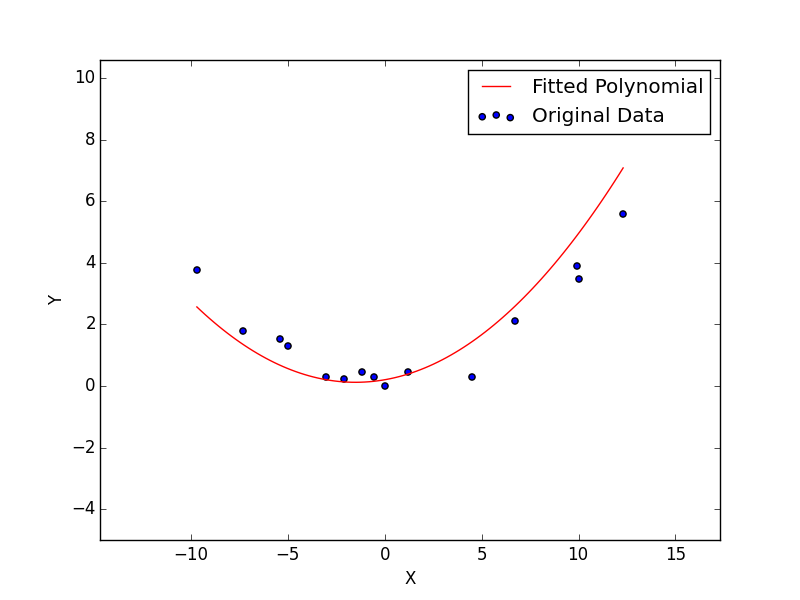
\includegraphics[scale=0.75]{Q1_fig.png}
    \caption{Plot showing the data points and the polynomial as determined by the algorithm. The polynomial has been evaluated at 100 equidistant points between [-9.7, 12.3] and the degree of the polynomial fit is 2}
	\label{fig:Q1_fig}
\end{figure}

% \begin{figure}[ht]
% 	\center
%     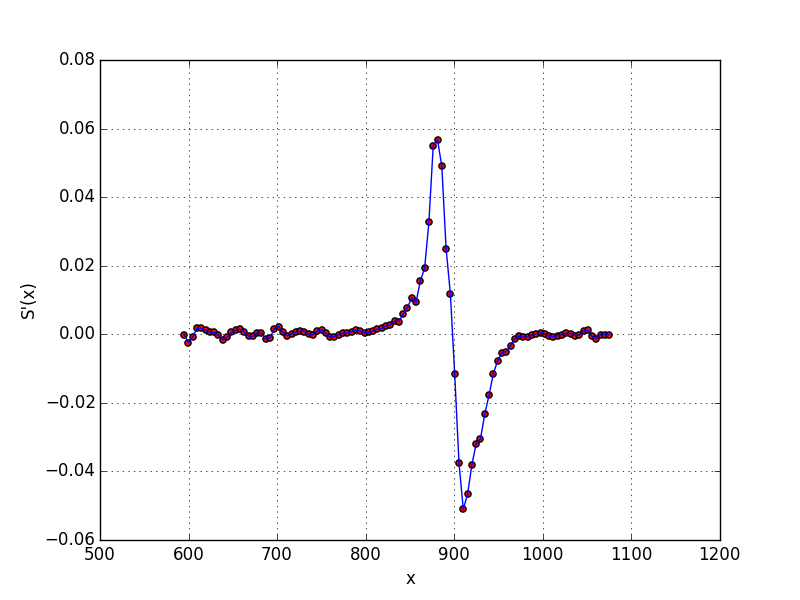
\includegraphics[scale=0.75]{plotS_dash.png}
%     \caption{Plot showing the first derivative of the natural cubic interpoland S'(X). Values of $S'(X_i)$ for $X_i$ in the range of (min(knot values), max(knot values)) are shown as red circles.} 
% 	\label{fig:sdash}
% \end{figure}


% \begin{table}[ht]
% \centering
% \label{my-label}
% \begin{tabular}{|c|c|c|}
% \hline
%  \textbf{n}&\textbf{RMS Error}&\textbf{Condition Number}  \\ \hline
%  2&0.73833521&15.0167409881  \\ \hline
%  5&1.02602254&282901.77002 \\ \hline
%  8&1.09505307&7657562245.89 \\ \hline
%  12&1.16783884&5.89342127254e+15 \\ \hline
%  15&2.11656192&1.74359790918e+17 \\ \hline
% \end{tabular}
% \caption{Table showing the values of n and the RMS error after solving the system of linear equations with \textbf{hilbert(n)} as the coefficients.}
% \end{table}
The corresponding python code can be found at \ref{code:problem3a}
\subsection{Fitting the polynomial regressor on \textit{World Population} data.}\label{prob3b}
In this question we are asked to repeat the polynomial regression as above, but on a different dataset. The dataset and the output of the algorithm can be found in Table 3 and Table 4 respectively.

In the figure below we have plotted the degree 4 polynomial as suggested by the algorithm. It can be seen that the polynomial does not fit the data very well.

This is because of the large set of missing values between years 1000 and 1650. Because of these missing values, the dataset doesn't represent the underlying trend very well, resulting in a bad polynomial fit.
 
Hence, polynomial regression is not very well suited to fit data with a lot of missing values, It should be used only when the dataset is fairly evenly spread through the range of values over which we want to fit the polynomial.

\textbf{NOTE:} In the subsequent section we evaluate the fit of the same data augmented with some dummy values between 1000 and 1650. To evaluate whether the fit of the polynomial regressor improves.
\begin{figure}[ht]
	\center
    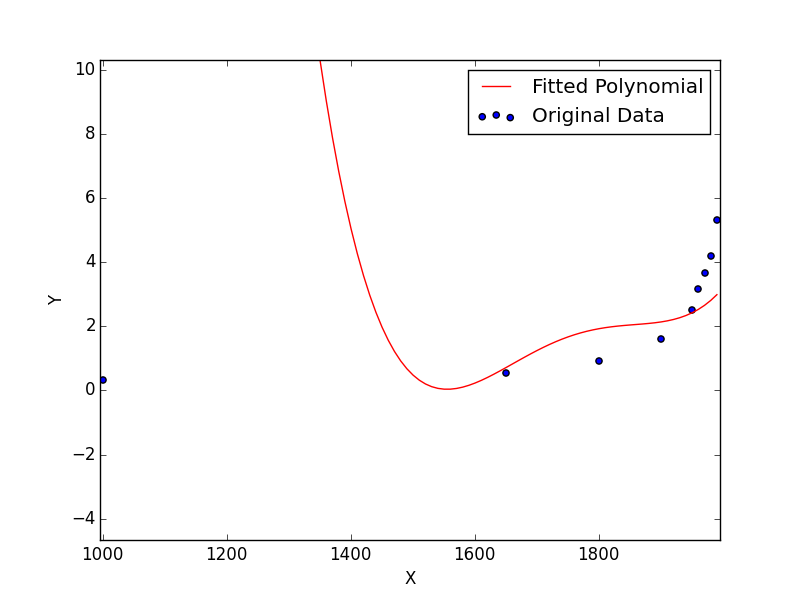
\includegraphics[scale=0.75]{Q1b_fig.png}
    \caption{Plot showing the World population dataset and the 4th degree polynomial as suggested by our algorithm. It can be visually verified that the data is not very well fit with the given 4th degree polynomial}
	\label{fig:world_pop}
\end{figure}

\begin{table}[ht]
\centering
\label{population-label}
\begin{tabular}{|c|c|}
\hline
 \textbf{x}&\textbf{y} \\ \hline
1000 & 0.34 \\
1650 & 0.545 \\
1800 & 0.907 \\
1900 & 1.61 \\
1950 & 2.51 \\
1960 & 3.15 \\
1970 & 3.65 \\
1980 & 4.2 \\
1990 & 5.3 \\
\hline
\end{tabular}
\caption{The \textit{World Population} dataset that needs to be fit with the polynomial regressor used in the previous section.}
\end{table}

\begin{table}[ht]
\centering
\label{polynomial-args}
\begin{tabular}{|c|c|c|c|c|}
\hline
 i &       alpha  &       beta    &  variance   &         c\\ \hline
 0 &  1800.000000 &    0.000000   &   3.035407  &   2.468000\\
 1 &  1201.833741 &  90888.888889 &    1.821713 &    0.003755\\
 2 &  1671.383205 &  58100.462442 &    0.714551 &    0.000013\\
 3 &  1811.975200 &  10318.358986 &    0.270872 &    0.000000\\
 4 &  1881.282629 &  6073.275792  &   0.063930  &   0.000000\\
\hline
\end{tabular}
\caption{Tabulated values of $i$ : the degree n of the polynomial. alpha($\alpha$) and beta($\beta$) : The corresponding multipliers used to generate the nth degree polynomial in the equation \\ $q_{n+1}(x) = xq_{n}(x) - \alpha_n q_{n}(x) - \beta_n q_{n-1}(x)$ \and Finally c : is the coefficient used in evaluating the polynomial $p_{n}(x) = \sum_{i=0}^{n}c_{i}q_{i}$ these values are for the \textit{World Population} dataset. Here the algorithm computes that a polynomial of degree 4 would be the best fit for the given data.}
\end{table}
\clearpage
\subsubsection{Augmenting the world population data with dummy values to check if the overall fit of the polynomial regressor improves.}\label{augmented_section}
% Augmented data
In this section, we run a small experiment to check if the overall fit of the polynomial regressor improves if the dataset has fewer gaps ( missing values ).

For the experiment, we have augmented the \textit{World Population dataset} with a few dummy values between years 1000 and 1650. The new dataset is given in Table 5. 



\begin{table}[ht]
\centering
\label{augmented-label}
\begin{tabular}{|c|c|}
\hline
 \textbf{x}&\textbf{y} \\ \hline
1000 & 0.34 \\
1100 & 0.38 \\
1200 & 0.42 \\
1300 & 0.5 \\
1450 & 0.51 \\
1650 & 0.545 \\
1800 & 0.907 \\
1900 & 1.61 \\
1950 & 2.51 \\
1960 & 3.15 \\
1970 & 3.65 \\
1980 & 4.2 \\
1990 & 5.3 \\
\hline
\end{tabular}
\caption{The \textit{World Population} dataset \textbf{\textit{augmented with dummy data}}  between years 1000 and 1650 to check the hypothesis that adding in the missing values indeed results in a polynomial regressor which has a better fit to the overall data.}
\end{table}
We run the same polynomial regression algorithm on the new dataset and find that a 4th degree polynomial would give the smallest least squares error with the augmented dataset. The output of the algorithm can be seen in Table 6.

\begin{table}[ht]
\label{table:polynomial_args_3}
\centering
\begin{tabular}{|c|c|c|c|c|}
\hline
 i &       alpha  &       beta     &  variance &         c\\ \hline
 0 &  1634.615385 &    0.000000    &  2.962034 &   1.847846\\
 1 &  1443.872563 &  129609.467456 &  1.225232 &  0.003619\\
 2 &  1433.542239 &  49394.313405  &  0.671342 &  0.000009\\
 3 &  1478.542841 &  67784.468510  &  0.342014 &  0.000000\\
 4 &  1492.567253 &  58694.769631  &  0.187048 &  0.000000\\
\hline
\end{tabular}
\caption{Tabulated values of $i$ : the degree n of the polynomial. alpha($\alpha$) and beta($\beta$) : The corresponding multipliers used to generate the nth degree polynomial in the equation \\ $q_{n+1}(x) = xq_{n}(x) - \alpha_n q_{n}(x) - \beta_n q_{n-1}(x)$ \and Finally c : is the coefficient used in evaluating the polynomial $p_{n}(x) = \sum_{i=0}^{n}c_{i}q_{i}$ these values are for the \textit{World Population} dataset \textit{\textbf{augmented with dummy data}} to test the hypothesis that adding the missing data between years 1000 and 1650 gives a better polynomial regressor for the entire dataset. Here the algorithm computes that a polynomial of degree 4 would be the best fit for the data.}
\end{table}

We see that visually overall fit of the 4th degree polynomial to the augmented dataset looks much better. See \ref{fig:test_fig}

\begin{figure}[ht]
	\center
    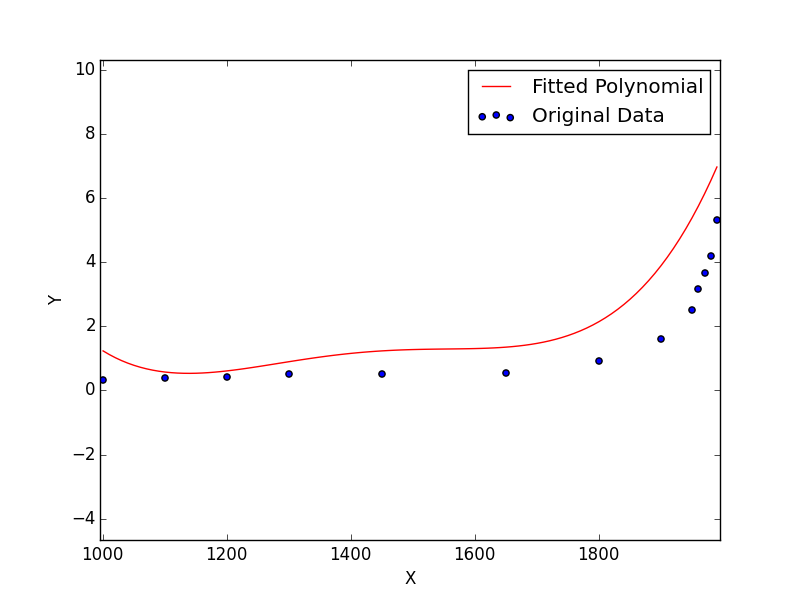
\includegraphics[scale=0.75]{Q1b_test_fig.png}
    \caption{Plot showing the augmented data and the polynomial regressor. It can be visually verified that this fit is better than the one in which the data between years 1000 and 1650 were missing.}
	\label{fig:test_fig}
\end{figure}


% \begin{figure}[ht]
% 	\center
%     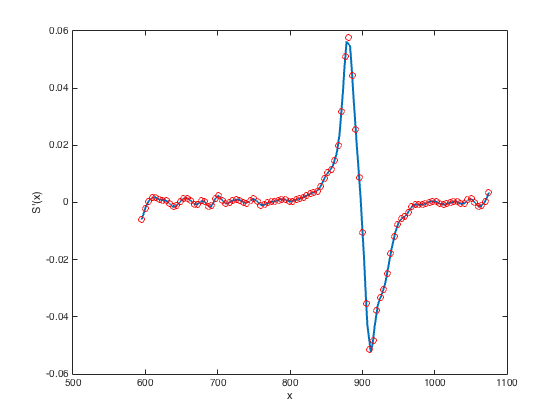
\includegraphics[scale=0.75]{matlabS_dash.png}
%     \caption{Plot showing the first derivative of the natural cubic interpoland S'(X) as calculated using Matlab. Values of $S'(X_i)$ for $X_i$ in the range of (min(knot values), max(knot values)) are shown as red circles.} 
% 	\label{fig:sdash_matlab}
% \end{figure}
% The corresponding plots created by matlab are much more smoother because matlab implements an additional constraint that the third derivatives of the piecewise polynomials are also equal at the second and the last knots. This are apparently called the "Not-A-Knot" end conditions. This is only done when the length of \textbf{t} and \textbf{y} are same.
% 
% Natural splines are a good choice only when the functions have 0 second derivative at the end points. I read it up from here. \url{http://www.mathworks.com/matlabcentral/newsreader/view_thread/172988} would really appreciate some more information about why using the Not-A-Knot condition is better. 
% \\
% The corresponding matlab code can be found at \ref{code:problem2b}
\clearpage

\section{Appendix A}\label{code:problem3a}
Python source code for \ref{prob3a} and \ref{prob3b}.
{\footnotesize
\begin{lstlisting}
import numpy as np
import pylab as pl

def dot_prod(x,y):
    # the lenght of arrays must be same.
    assert(len(x) == len(y))
    # get corresponding values from x and y 
    # for v in zip(x,y)
    # find their product and put the result in a list, list comprehension.
    # sum over the list
    return np.sum([v[0]*v[1] for v in zip(x,y)])

def get_next_alpha(x,qPrev):
    # Caclulating new alpha now
    alpha_num = dot_prod(x*qPrev,qPrev)
    alpha_denom = dot_prod(qPrev,qPrev)
    return np.true_divide(alpha_num, alpha_denom) 

def get_next_beta(x,qPrev,qOld):
    # Calculating new beta now
    beta_num = dot_prod(x*qPrev,qOld) # beta's numerator
    beta_denom = dot_prod(qOld,qOld) # beta's denominator
    return np.true_divide(beta_num, beta_denom) 

def get_parameters(x,y):
    m = len(x) - 1
    # qi-2
    qOld = np.ones(x.shape)

    # Initial alpha alues
    alpha = np.zeros(x.shape)
    alpha[0] = np.true_divide(dot_prod(x * qOld, qOld),dot_prod(qOld,qOld))

    # allocating space for beta
    beta = np.zeros(x.shape)

    # qi-1
    qPrev = x - alpha[0]

    # Initializing c
    c = np.zeros(x.shape)
    c[0] = np.true_divide(dot_prod(y,qOld),dot_prod(qOld,qOld))
    c[1] = np.true_divide(dot_prod(y,qPrev),dot_prod(qPrev,qPrev))

    # Rho i and i-1
    rho = np.ones(x.shape)
    rho[0] = dot_prod(y,y) - np.true_divide(np.square(dot_prod(y,qOld)),dot_prod(qOld,qOld))
    rho[1] = rho[0] - np.true_divide(np.square(dot_prod(y,qPrev)),dot_prod(qPrev,qPrev))

    # Start with degree 1
    n = 1 

    # Initializing sigma_sq
    sigma_sq = np.ones(x.shape)
    sigma_sq[0] = np.true_divide(rho[0], m)
    sigma_sq[1] = np.true_divide(rho[1], m-n) 
    while(True):
        # Calculating new beta now
        beta[n] = get_next_beta(x,qPrev,qOld)
        
        # Caclulating new alpha now
        alpha[n] = get_next_alpha(x,qPrev)

        # Calculating q_n+1
        qNew = x*qPrev - alpha[n]*qPrev - beta[n]*qOld

        # Calculating new C
        c[n+1] = np.true_divide(dot_prod(y,qNew),dot_prod(qNew,qNew))

        # Calculate rho_n+1
        rho[n+1] = rho[n] - np.true_divide(np.square(dot_prod(y,qNew)),dot_prod(qNew,qNew))
        # Calculate sigma_sq_n+1
        sigma_sq[n+1] = np.true_divide(rho[n+1],m-(n+1))
        # if sigma_sq_n+1 > sigma_sq_n 
        # or abs(sigma_sq_n - sigma_sq_n+1) < 0.1
        # Then stop
        if sigma_sq[n+1] > sigma_sq[n] or np.abs(sigma_sq[n] - sigma_sq[n+1]) < 0.1:
            break
        else:
            # Update n += 1
            n += 1
            # update qOld,qPrev = qPrev,qNew
            np.copyto(qOld,qPrev)
            np.copyto(qPrev,qNew)
    
    return c,alpha,beta,sigma_sq,n

def evaluate(t,alpha,beta,c,n):
    x_vals = np.asarray(t)
    retVals = []
    for x in x_vals:
        sum = 0
        # qi-2
        qOld = np.ones(1)
        sum += c[0]*qOld
        # qi-1
        qPrev = x - alpha[0]
        sum += c[1]*qPrev
        for i in range(2,n+1): # 2,n+1 because 0 and 1 are already calculated
            qNew = x*qPrev - alpha[i]*qPrev - beta[i]*qOld
            qOld = qPrev
            qPrev = qNew
            sum += c[i] * qNew
        retVals.append(sum)
    return retVals

def process_and_plot(data,pl,file_name=None):
    x,y = map(np.asarray,zip(*data))
    c,alpha,beta,sigma_sq,n = get_parameters(x,y)
    
    print("\n{:>2} {:>10} {:>10} {:>10} {:>10}".format("i","alpha","beta","variance","c"))
    for i in range(n+1):
        print("{:2d} {:10f} {:10f} {:10f} {:10f}".format(i,alpha[i],beta[i],sigma_sq[i],c[i]))
        # print(i,alpha[i],beta[i],sigma_sq[i],c[i])

    pl.scatter(x,y,label="Original Data")
    xvals = np.linspace(min(x),max(x),100)
    yvals = evaluate(xvals,alpha,beta,c,n)
    pl.plot(xvals,yvals,c='r',label="Fitted Polynomial")
    pl.xlim(min(x)-5,max(x)+5)
    pl.ylim(min(y)-5,max(y)+5)
    pl.xlabel("X")
    pl.ylabel("Y")
    pl.legend()
    if file_name != None:
        pl.savefig(file_name)

if __name__ == '__main__':
    # Q3.a data
    data = [(-9.70,3.76),
            (-7.30,1.78),
            (-5.40,1.52),
            (-5.00,1.31),
            (-3.01,0.31),
            (-2.13,0.23),
            (-1.20,0.45),
            (-0.56,0.29),
            (0.00,0.00),
            (1.20,0.45),
            (4.50,0.28),
            (6.70,2.12),
            (9.90,3.91),
            (10.00,3.47),
            (12.30,5.59)]
    pl.figure()
    process_and_plot(data,pl,"Q1_fig.png") 
    # test data, almost straight line
    data_2 = [(1,4),(2,4.5),(3,3.9),(4,4.6),(4,3.7)]
    pl.figure()
    process_and_plot(data_2,pl)
    # Q3.b data
    data_3 = [(1000,0.340),(1650,0.545),(1800,0.907),(1900,1.61),(1950,2.51),(1960,3.15),(1970,3.65),(1980,4.20),(1990,5.30)]
    pl.figure()
    process_and_plot(data_3,pl,"Q1b_fig.png")
    # Q3.b test data
    test_data = [(1000,0.340),(1100,0.38),(1200,0.42),(1300,0.5),(1450,0.51),(1650,0.545),(1800,0.907),(1900,1.61),(1950,2.51),(1960,3.15),(1970,3.65),(1980,4.20),(1990,5.30)]
    pl.figure()
    process_and_plot(test_data,pl,"Q1b_test_fig.png")

    pl.show()
    pl.close()
\end{lstlisting}
}
\end{document}


